\documentclass[10pt,twoside,slovak,a4paper]{article}

\usepackage[slovak]{babel}
%\usepackage[T1]{fontenc}
\usepackage[IL2]{fontenc} 
\usepackage[utf8]{inputenc}
\usepackage{graphicx}
\usepackage{amsmath}
\usepackage{wrapfig}
\usepackage{url} % príkaz \url na formátovanie URL
\usepackage{hyperref} 

\usepackage{cite}
%\usepackage{times}

\pagestyle{headings}

\title{Problems of recommendation systems and their uncertain future\thanks{Semestrálny projekt v predmete Metódy inžinierskej práce, ak. rok 2024/25, vedenie: Yevheniia Kataieva }} 

\author{Dmytro Panychuk\\[2pt]
	{\small Slovenská technická univerzita v Bratislave}\\
	{\small Fakulta informatiky a informačných technológií}\\
	{\small \texttt{xpanychuk@stuba.sk}}
	}

\date{\small 28. oktober 2024} 

\begin{document}

\maketitle

\begin{abstract}
\centering


Recommendation systems have become an incredibly important part of our lives. They are used in all online services, and the frequency of their use is only growing every year. 

These algorithms are used to personalise the experience by making suggestions tailored to our preferences and interests. The use of such systems is beneficial for both the platform and the end user. It recommends products that the user is more likely to buy, which saves them time and the platform will receive additional profit from new sales.  Without them, our modern online world would be impossible because it is a thing that allows the customer to find the product they need and the seller to increase sales through the target audience.

But these systems cannot be effective without users' personal information. This causes a lot of problems, both legal and moral. On the one hand, the user is not fully aware of how much of their personal information the platform receives, and on the other hand, databases are often hacked and your personal information can become public in a matter of seconds.

Also, the results of these systems are not always predictable. Sometimes, using recommendation systems can lead you into an “information bubble” from which you cannot get out without help. This can lead to terrible consequences that have already happened many times in human history. 

In this article, we will look at the problems of recommendation systems and the situations they have led to. We will also explore the methods of dealing with these problems that are used now and will be used in the future.
\newpage

\end{abstract}



\section{Introduction}
In today's information society, where the amount of data and information is growing exponentially, users often face the problem of information overload\cite{overload}. This phenomenon, known as ‘information overload’, makes it difficult to find the right products and services. In turn, sellers face difficulties in promoting their products in a competitive environment\cite{business}. Therefore, recommendation systems have become an integral part of modern business\cite{comerce}, as their main goal is to efficiently sort and select products according to individual user preferences.

Recommendation systems operate based on the analysis of user behavior, purchase history, product ratings and other factors. They use algorithms to predict whether a particular product is likely to appeal to a particular user based on previous preferences. In the digital world, such systems have become important tools for increasing customer satisfaction and driving sales for large e-commerce companies\cite{store}.

Well-implemented recommendation systems can significantly improve the user experience by making the shopping process more personalized\cite{closeness} and convenient. They help customers find the right products faster and expand their choices, which in turn helps to increase sales for businesses\cite{comerce}. Given these factors, the implementation of recommendation systems has become imperative for the successful operation of modern businesses.


While much has been written about the benefits of recommendation systems, the negative aspects of their use remain less well understood. These may include data privacy issues, algorithmic bias, and the risk of creating ‘information bubbles’ where users only receive content that confirms their existing views. This can lead to a limited diversity of information and products, which can negatively impact the user experience.

In this article, I plan to first describe in detail the general principles of recommendation systems~\ref{How They Work}, and then consider their varieties~\ref{Types of recommendation systems}, such as content-based recommendations, collaborative filtering, and hybrid approaches. Next, I will analyse the benefits that recommendation systems can provide to both users~\ref{Benefits for Users} and businesses~\ref{Benefits for Platforms}, highlighting their role in increasing customer satisfaction and sales performance.

Finally, I will focus on the challenges associated with recommendation systems~\ref{Ethical and Legal Issues} ~\ref{Risks of Data Breaches} ~\ref{Information Bubbles} and try to find possible solutions to these problems~\ref{Current and Future Solutions} ~\ref{Conclusion}. My suggestions will be based on research and innovations already being implemented by various companies and governments. This will include discussions on ethical standards, transparency of algorithms, and ways to ensure diversity in recommendations for users.




\section{How They Work} \label{How They Work}
The general principle of recommendation systems is to analyze user preferences and behaviors in order to suggest relevant items, products, or content. These systems aim to enhance the user experience by providing personalized recommendations based on various data sources.

\begin{itemize}
\newpage
\item \textbf{Data Collection}

Recommendation systems gather data from users, which can include explicit feedback (such as ratings and reviews), implicit feedback (such as browsing history, purchase history, and time spent on items), and demographic information.
\item \textbf{User Profiling}

Based on the collected data, the system creates a profile for each user. This profile reflects the user’s preferences, interests, and behaviors.
\item \textbf{Item Representation}

 Items in the system are also represented in a way that captures their features. This can involve various attributes, such as genre for movies, categories for products, or keywords for articles.
\item \textbf{Output Recommendations}

 After processing the data through the algorithms, the system generates a list of recommended items tailored to each user. This list is presented to the user through various interfaces, such as online stores, streaming services, or social media platforms.
 \item \textbf{Feedback Loop}
 
 As users interact with the recommendations (by clicking, purchasing, or rating), the system continuously updates user profiles and item representations, refining its recommendations over time. This iterative process enhances the personalization of the system.
\end{itemize}

In summary, recommendation systems work by collecting user and item data, analyzing it through algorithms, and providing personalized suggestions, ultimately aiming to improve user satisfaction and engagement.



 \begin{figure}[!h]
    \centering
    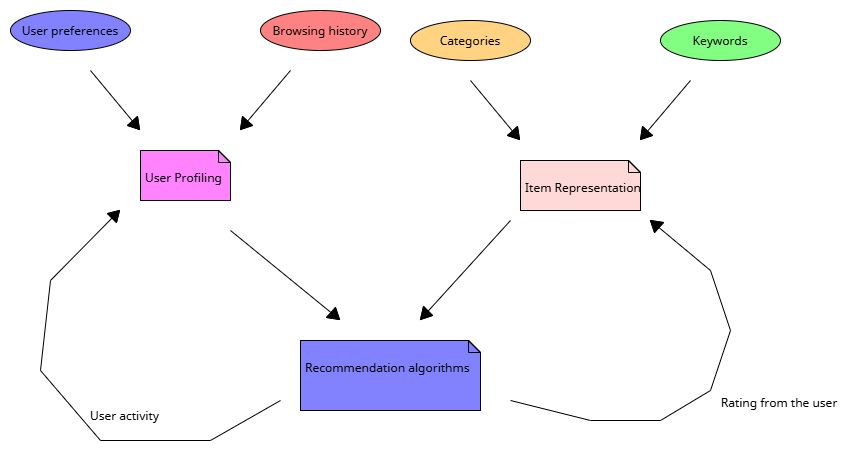
\includegraphics[width=1\linewidth]{Diagram 2.png}
    \caption{How the recommendation system works}
    \label{fig:recommendations}
\end{figure}
 


\newpage
\section{Types of recommendation systems} \label{Types of recommendation systems}

In general, recommendation systems are divided into two types: Collaborative Filtering and Content-Based Filtering\cite{types}.

\begin{enumerate}
\item  \textbf{Collaborative Filtering}

Collaborative filtering relies on the idea that users who agreed in the past will agree in the future. The system finds two people with similar user profiles and recommends to one of them what the other liked, expecting that he will like it too, because they have similar interests.
\begin{figure}[!h]
    \centering
    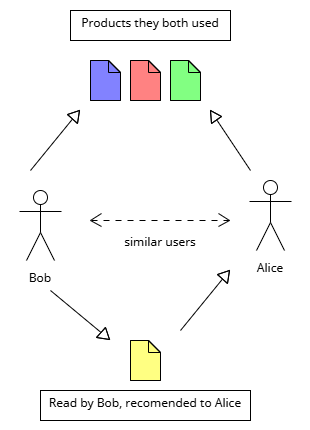
\includegraphics[width=0.8\linewidth]{Diagram 3.png}
    \caption{Collaborative Filtering Diagram}
    \label{fig:collaborative}
\end{figure}

\newpage
\item  \textbf{Content-Based Filtering}

Content-based filtering focuses on the characteristics of the items themselves rather than on user interactions. If the user has chosen items in the past that were somewhat similar to each other, the system will recommend things that also have something in common with them, expecting the user to like it because he liked it in the past.
\begin{figure}[!h]
    \centering
    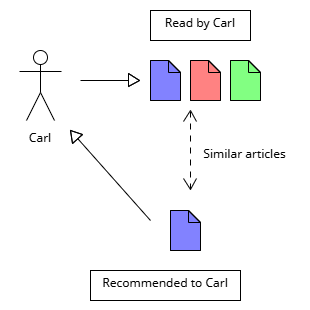
\includegraphics[width=0.7\linewidth]{Diagram 4.png}
    \caption{Content-based Filtering Diagram}
    \label{fig:content-based}
\end{figure}
	
\end{enumerate}

But the most effective method is to combine these two types. This allows you to create personalised recommendations based on both a person's past actions and the actions of people with similar preferences. Such recommendations are best suited to the user's preferences.


\section{Benefits for Users} \label{Benefits for Users}
Users gain several significant benefits from recommendation systems that enhance their experience with products and services. First, these systems provide personalization by offering recommendations based on user preferences and behavior, helping users find items or content that best match their individual tastes.

Second, thanks to automated recommendations, users can save time by quickly locating what they need without having to sift through a vast amount of information. This makes the process of shopping or searching for content more efficient. Additionally, recommendation systems open up new possibilities by helping users discover products or services they might not have found on their own, including new brands, genres, or categories.

Moreover, personalized recommendations increase user satisfaction, as they boost the likelihood that a user will find something they enjoy, which, in turn, enhances overall enjoyment of the purchase or content consumption. Recommendation systems also reduce information overload by filtering through large amounts of available information, helping users avoid stress when choosing from numerous options.

For example in this study \cite{closeness}using the following formulas

\begin{eqnarray}
    &&\begin{array}{*{35}{l}}
        s_{\alpha \beta}^{\left(\text{CN}\right)}(t)=\underset{i=0}{\overset{N}{\sum}}\,{{a}_{i\alpha}}(t){{a}_{i\beta}}(t), 
    \end{array}
\end{eqnarray}

\begin{eqnarray}
    &&\begin{array}{*{35}{l}}
        s_{\alpha \beta}^{\left(\text{cosine}\right)}(t)=\frac{1}{\sqrt{{{k}_{\alpha}}{{k}_{\beta}}}}\underset{i=0}{\overset{N}{\sum}}\,{{a}_{i\alpha}}(t){{a}_{i\beta}}(t). 
    \end{array}
\end{eqnarray}

researchers have determined that
sufficiently effective systems can increase the accuracy of recommendations for the buyer several times.
\begin{figure}[!h]
    \centering
    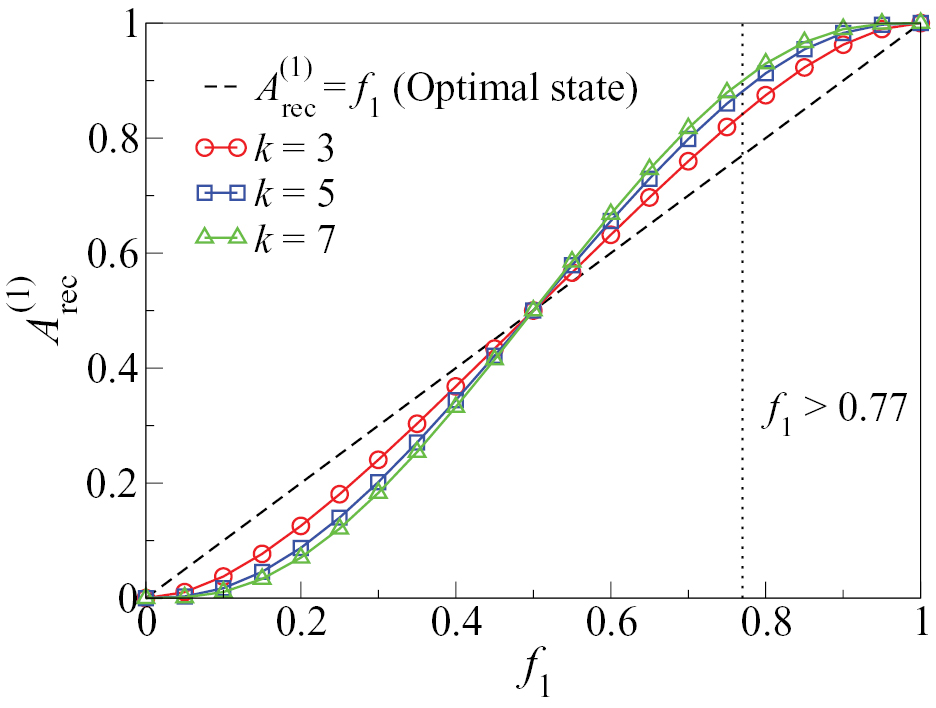
\includegraphics[width=0.9\linewidth]{picture.jpg}
    \caption{closeness of the recommended to the desired result}
    \label{fig:closeness}
\end{figure}

Furthermore, users who receive relevant recommendations are more likely to engage with the platform, which can lead to repeat purchases or more frequent use of services. In some systems, the opinions of friends or other users are taken into account, allowing for recommendations based on social connections and increasing trust in specific products or services.

Finally, recommendation systems can adapt to changes in user preferences by incorporating new data and feedback, ensuring that recommendations remain relevant. In summary, recommendation systems create a more convenient, efficient, and satisfying experience for users, allowing them to find what truly aligns with their interests and needs.



\newpage
\section{Benefits for Platforms} \label{Benefits for Platforms}
Companies gain numerous advantages from implementing recommendation systems, which can significantly enhance their business performance. First and foremost, these systems contribute to increased sales by suggesting relevant products that users may want to purchase, stimulating impulse buys and raising the average transaction value.

Additionally, personalized recommendations improve overall customer satisfaction, leading to a higher level of customer contentment. Satisfied customers are more likely to return and recommend the company to others, fostering positive word-of-mouth. Moreover, when users receive tailored suggestions that align with their interests, the likelihood of cart abandonment decreases, which is especially crucial in a competitive market.

Recommendation systems also help build customer loyalty by creating a closer connection between users and the brand. When a company offers relevant content or products, it fosters brand loyalty among its customers. Furthermore, the data analyzed by these systems provides valuable insights into customer behavior and preferences, allowing companies to refine their marketing strategies effectively.

By enabling more precise targeting in marketing campaigns, recommendation systems can optimize marketing expenditures, reducing costs while increasing effectiveness. Recommendations based on user interests can lead to higher conversion rates, making marketing efforts more efficient.

Moreover, companies that successfully implement effective recommendation systems can gain a competitive edge in the market by offering a more personalized experience compared to their rivals. This competitive advantage can be crucial in attracting and retaining customers.

Finally, personalized recommendations can encourage users to spend more time on the platform, which may lead to increased purchases or content consumption. In summary, recommendation systems not only enhance user experience but also provide substantial business benefits, such as increased sales, reduced marketing costs, and strengthened customer loyalty. Implementing such systems is becoming an essential element of successful business strategy in today’s competitive environment.

\section{Ethical and Legal Issues} \label{Ethical and Legal Issues}

\section{Risks of Data Breaches} \label{Risks of Data Breaches}

\section{Information Bubbles} \label{Information Bubbles}
 

\section{Current and Future Solutions} \label{Current and Future Solutions}

\begin{table}[ht]
\centering
    \begin{tabular}{l|r}
        Year  & Billions of USD \\\hline
        2022  & 2.18  \\
        2023  & 2.8   \\
        2024  & 3.6   \\
        2025  & 4.63  \\
        2026  & 5.94  \\
        2027  & 7.64  \\
        2028  & 9.81   \\
        2029  & 12.61  \\
        2030  & 16.21  \\
        2031  & 20.82  \\
        2032  & 26.76  \\
        2033  & 34.39  \\
    \end{tabular}
    \caption{Finances to be invested in recommendation systems}
    \label{tab:widgets}
\end{table}
\section{Conclusion} \label{Conclusion}


%\acknowledgement{Ak niekomu chcete poďakovať\ldots}
\newpage
\bibliography{literatura}
\bibliographystyle{plain}
\end{document}
